% Remplacer les apostrophes ’ par des quotes '

{\setbeamerfont{framesubtitle}{size=\tiny}
\begin{frame}{\fe{Exercice 2 : fissuration par suppression d'éléments}
                 {Exercise 2: fracture by elements removal}}
             {\url{https://www-cast3m.cea.fr/index.php?page=exemples&exemple=formation_pasapas_2_initial}}
  \small
  \begin{itemize}
    \item \fe{Plaque en traction \textcolor{green}{(déplacements imposés)}}
             {Plate under tension \textcolor{green}{(imposed displacements)}}\\
    \vspace{0.2cm}
    \begin{center}
      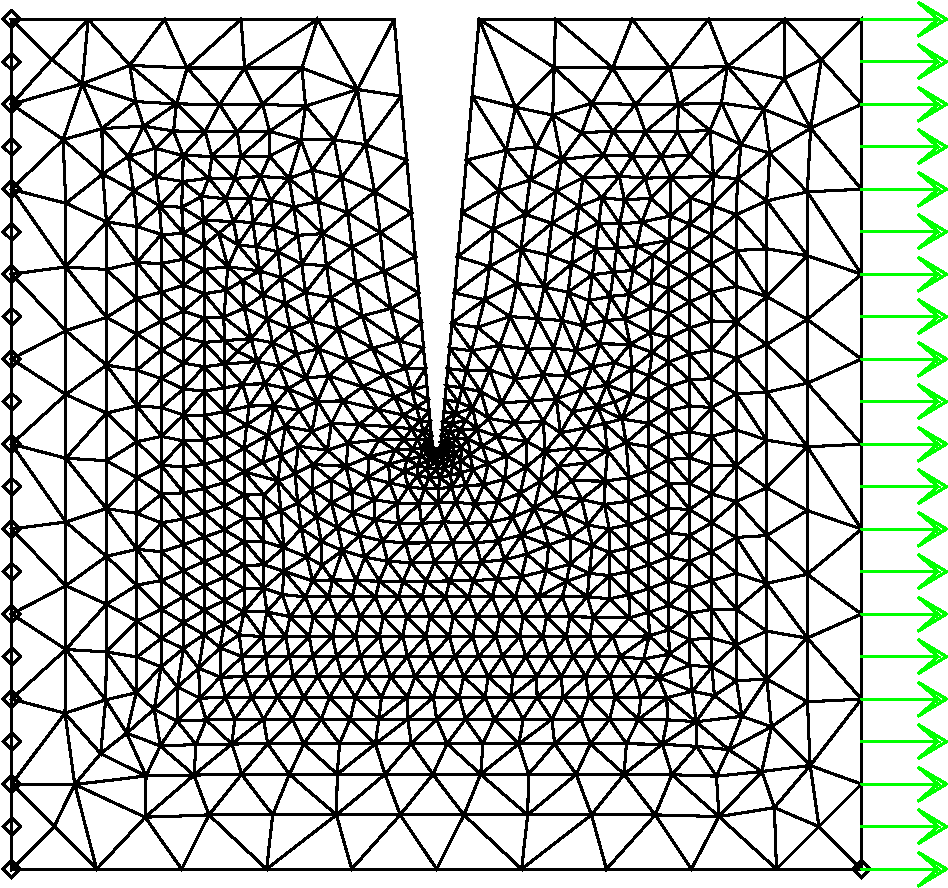
\includegraphics[height=3cm]{images/exo/exo_2_chargement}
      \hspace{0.1cm}
      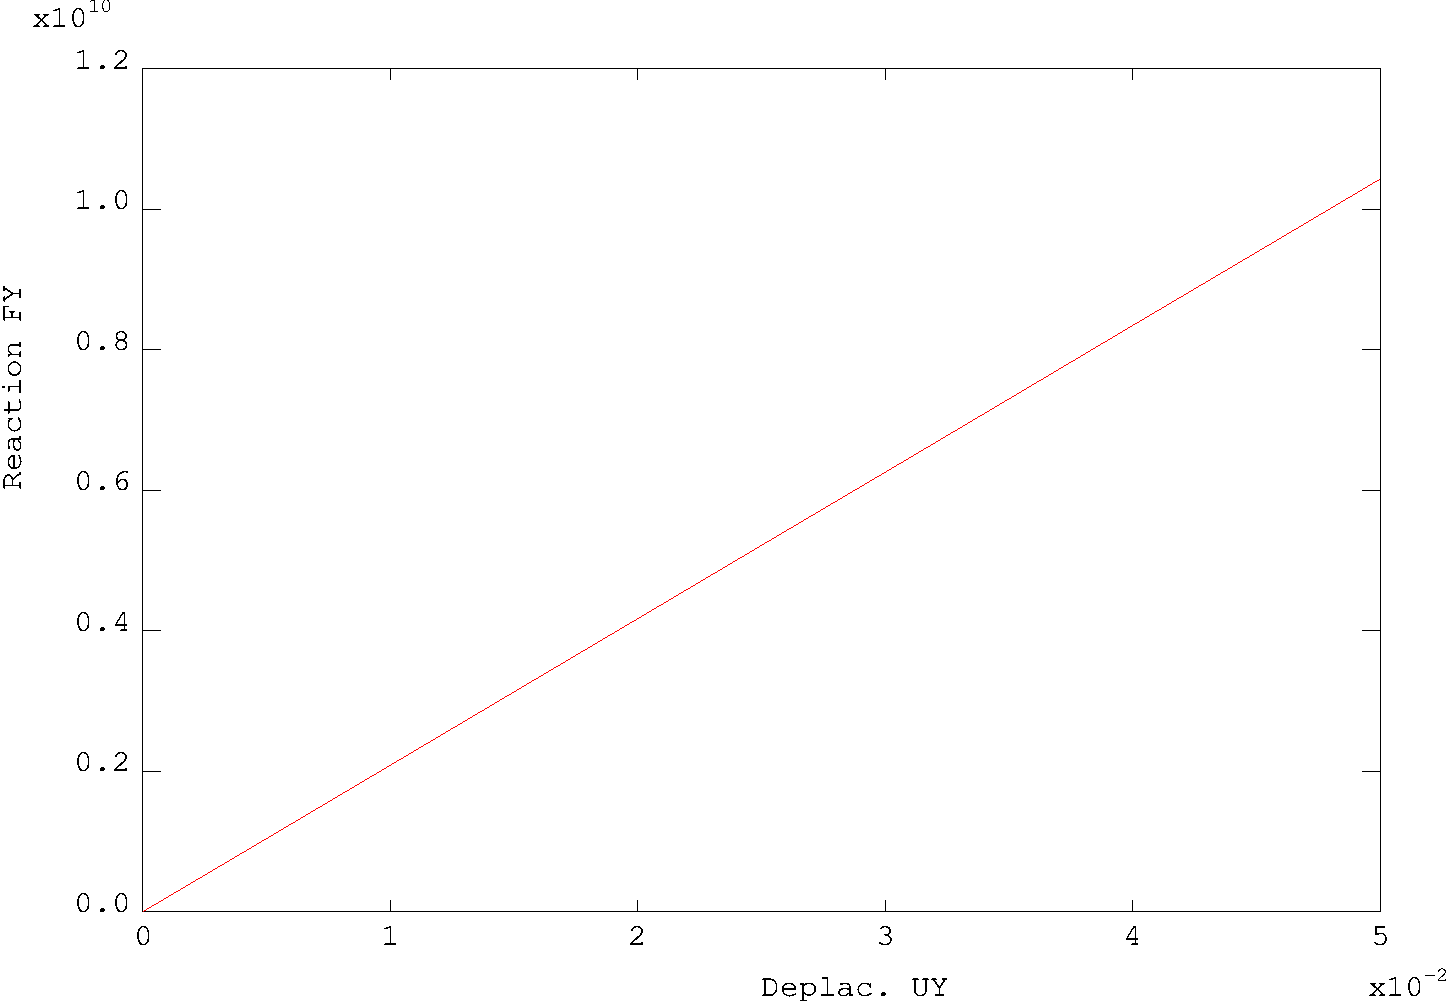
\includegraphics[height=3cm]{images/exo/exo_2_evol}
      \hspace{0.1cm}
      \animategraphics[controls,loop,poster=last,height=3cm]{10}{images/exo/exo_2_sigma.}{01}{10}
    \end{center}
    \item<2-> \fe{\green{Objectif : modéliser la rupture en \tou{supprimant les éléments} au cours du calcul}\\
                  On utilisera un critère simple sur la 1ère contrainte principale :
                  \begin{center}
                    rupture si $\sigma_I \geq$ 22~GPa\\ \avous{~À vous de jouer !}
                  \end{center}}
                 {\green{Purpose: to model fracture by \tou{removing elements} during calculations}\\
                  We will use a simple criterion based on the 1st principal stress:
                  \begin{center}
                    fracture if $\sigma_I \geq$ 22~GPa\\ \avous{~It's up to you!}
                  \end{center}}
  \end{itemize}
\end{frame}
}

{\setbeamerfont{framesubtitle}{size=\tiny}
\begin{frame}{\fe{Exercice 2 : fissuration par suppression d'éléments}
                 {Exercise 2: fracture by elements removal}}
             {\url{https://www-cast3m.cea.fr/index.php?page=exemples&exemple=formation_pasapas_2_initial}}
  \begin{itemize}
    \item \fe{Quelques opérateurs utiles}{Some useful operators}\\
    \small
    \kwr{PRIN} \fe{calcul des contraintes principales}{compute principal stresses}\\
    \kwr{ELEM} \fe{séléction des éléments où un champ vérifie une condition}{select the elements of a field that meets a criteria}\\
    \kwr{REDU} \fe{réduction d'un modèle sur un sous maillage}{reduction of a model on a sub part of a mesh}\\
    \kwr{CHAN} \fe{changement des points support d'un champ}{change the support points of a field}
    \normalsize
    \item \fe{Quelques indices utiles de la table}{Some useful table indices}\\
    \small
    \kwg{'ESTIMATION'.'CONTRAINTES'} \fe{dernier champ de contraintes convergé}{last converged stress field}
    \kwg{'WTABLE'.'MODELE'} \fe{modèle courant}{current model}\\
    \kwg{'WTABLE'.'CARACTERISTIQUES'} \fe{paramètres matériau}{material properties}
    \normalsize
  \end{itemize}
\end{frame}
}

\begin{frame}{\fe{Exercice 2 : fissuration par suppression d'éléments}
                 {Exercise 2: fracture by elements removal}}
             {\fe{Solution avec PERSO1}{Solution with PERSO1}}
  \footnotesize
  \begin{itemize}
    \small
    \item \fe{Utiliser la procédure \kwv{PERSO1}}{Use procedure \kwv{PERSO1}}
    \item \fe{Extraire le modèle et les contraintes dans \kwg{'ESTIMATION'}}{Extract the model and stress field in \kwg{'ESTIMATION'}}
    \item \fe{Calculer la contrainte principale $\sigma_I$}{Compute the 1st principal stress $\sigma_I$}
    \item \fe{Extraire les éléments "intacts"}{Extract the "intact" elements}
    \item \fe{Réduire le modèle sur ce maillage et écraser \kwg{'WTABLE'.'MODELE'}}
             {Reduce the model on this mesh and overwrite \kwg{'WTABLE'.'MODELE'}}
    \item \fe{Réduire les pas de temps}{Reduce time steps}
  \end{itemize}
  \vspace{4.5cm}
  \scriptsize
  \begin{textblock*}{10cm}(0.3cm,-3.2cm)
    \fe{\emph{Programme principal}}{\emph{Main program}}
    \lstinputlisting[basicstyle=\ttfamily\tiny, language=gibiane, firstline=92, lastline=95]{dgibi/formation_pasapas_2_solution.dgibi}
  \end{textblock*}
  \begin{textblock*}{10cm}(6.2cm,-4cm)
    \fe{\emph{\violet{Procédure PERSO1}}}{\emph{\violet{PERSO1 procedure}}}
    \lstinputlisting[basicstyle=\ttfamily\tiny, language=gibiane, firstline=75, lastline=84]{dgibi/formation_pasapas_2_solution.dgibi}
  \end{textblock*}
\end{frame}

\begin{frame}{\fe{Exercice 2 : fissuration par suppression d'éléments}
                 {Exercise 2: fracture by elements removal}}
             {\fe{Solution avec PERSO1}{Solution with PERSO1}}
  \footnotesize
  \begin{itemize}
    \item \fe{Résultats}{Results}
    \vspace{0.2cm}
    \begin{center}
      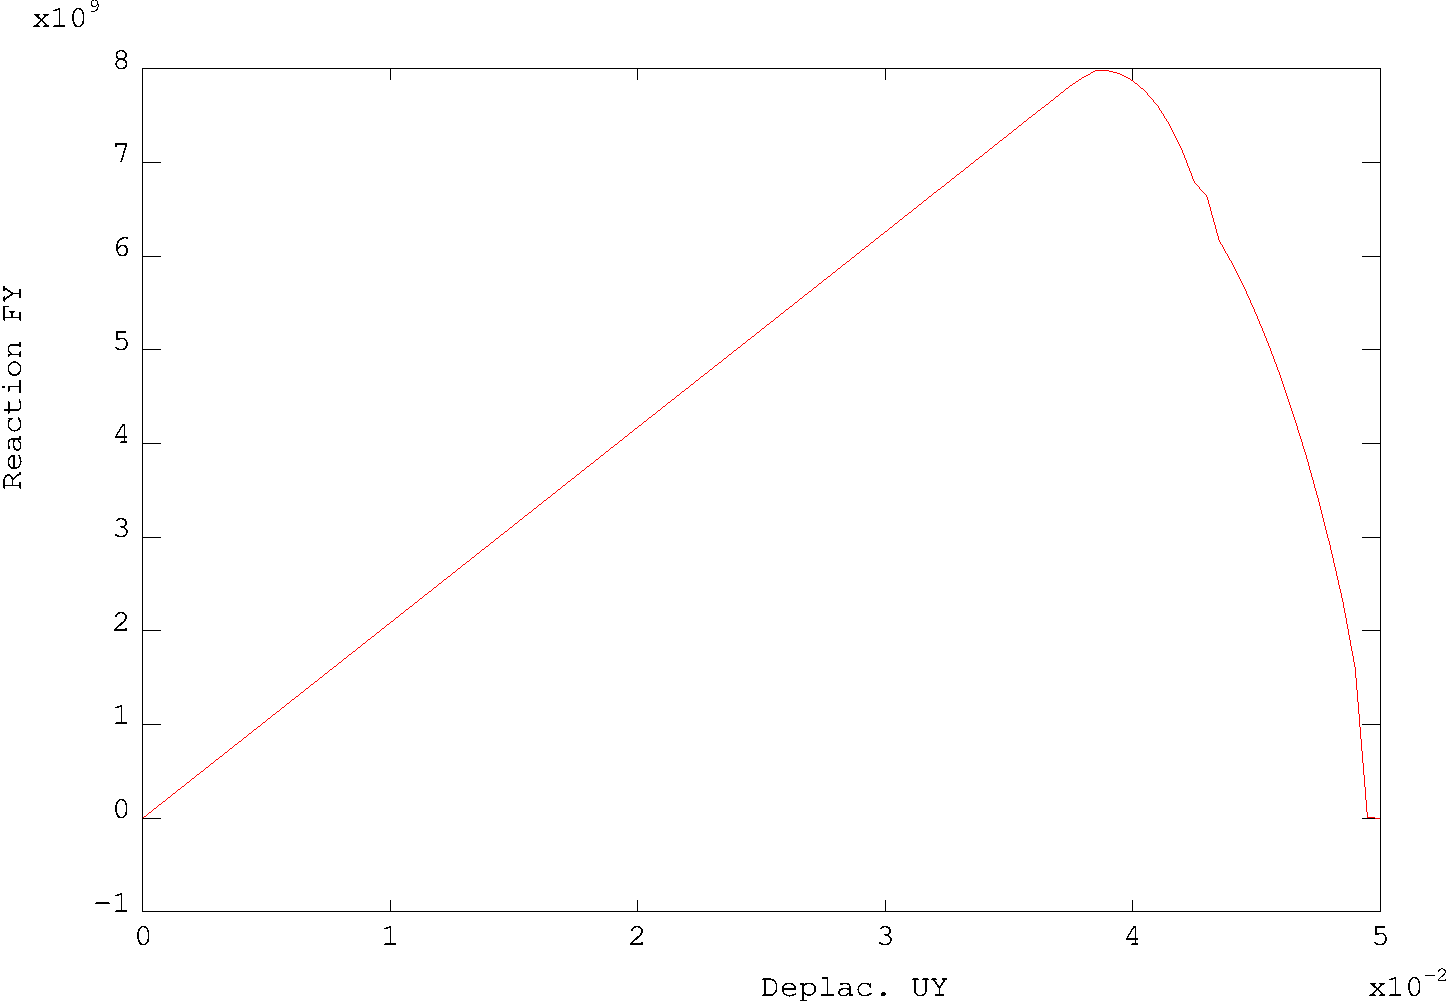
\includegraphics[height=3.5cm]{images/exo/exo_2_solu_evol}
      \hspace{0.4cm}
      \animategraphics[controls,loop,poster=last,height=3.5cm]{10}{images/exo/exo_2_solu_sigma.}{01}{46}
    \end{center}
    \item \fe{Modèle peu robuste\\ résultats très sensibles à la discrétisation espace/temps}
             {Undependable model\\ results quite sensitive to time/space discretization}
  \end{itemize}
\end{frame}

% \begin{frame}{\fe{Exercice 2 : fissuration par suppression d'éléments}
%                  {Exercise 2: fracture by elements removal}}
%              {\fe{Solution (bis) avec PERSO1}{Solution (bis) with PERSO1}}
%   \footnotesize
%   \begin{itemize}
%     \item \fe{Utiliser la procédure \kwv{PERSO1}}{Use procedure \kwv{PERSO1}}
%     \item \fe{Extraire le modèle et les contraintes dans \kwg{'ESTIMATION'}}{Extract the model and stress field in \kwg{'ESTIMATION'}}
%     \item \fe{Calculer la contrainte principale $\sigma_I$}{Compute the 1st principal stress $\sigma_I$}
%     \item \fe{Extraire les éléments "intacts"}{Extract the "intact" elements}
%     \item \fe{Réduire les \g{\red{blocages}} sur ce maillage} et écraser \kwg{'WTABLE'.'BLOCAGES\_MECANIQUES'}
%              {Reduce the \g{\red{boundary conditions}} on this mesh and overwrite \kwg{'WTABLE'.'BLOCAGES\_MECANIQUES'}}
%     \item \fe{Réduire les pas de temps}{Reduce time steps}
%   \end{itemize}
%   \vspace{4.5cm}
%   \scriptsize
%   \begin{textblock*}{10cm}(0.3cm,-3.2cm)
%     \fe{\emph{Programme principal}}{\emph{Main program}}
%     \lstinputlisting[basicstyle=\ttfamily\tiny, language=gibiane, firstline=92, lastline=95]{dgibi/formation_pasapas_2_solution.dgibi}
%   \end{textblock*}
%   \begin{textblock*}{10cm}(6.2cm,-4cm)
%     \fe{\emph{\violet{Procédure PERSO1}}}{\emph{\violet{PERSO1 procedure}}}
%     \lstinputlisting[basicstyle=\ttfamily\tiny, language=gibiane, firstline=75, lastline=84]{dgibi/formation_pasapas_2_solution.dgibi}
%   \end{textblock*}
% \end{frame}

% \begin{frame}{\fe{Exercice 2 : fissuration par suppression d'éléments}
%                  {Exercise 2: fracture by elements removal}}
%              {\fe{Solution (bis) avec PERSO1}{Solution (bis) with PERSO1}}
%   \footnotesize
%   \begin{itemize}
%     \item \fe{Résultats}{Results}
%     \vspace{0.2cm}
%     \begin{center}
%       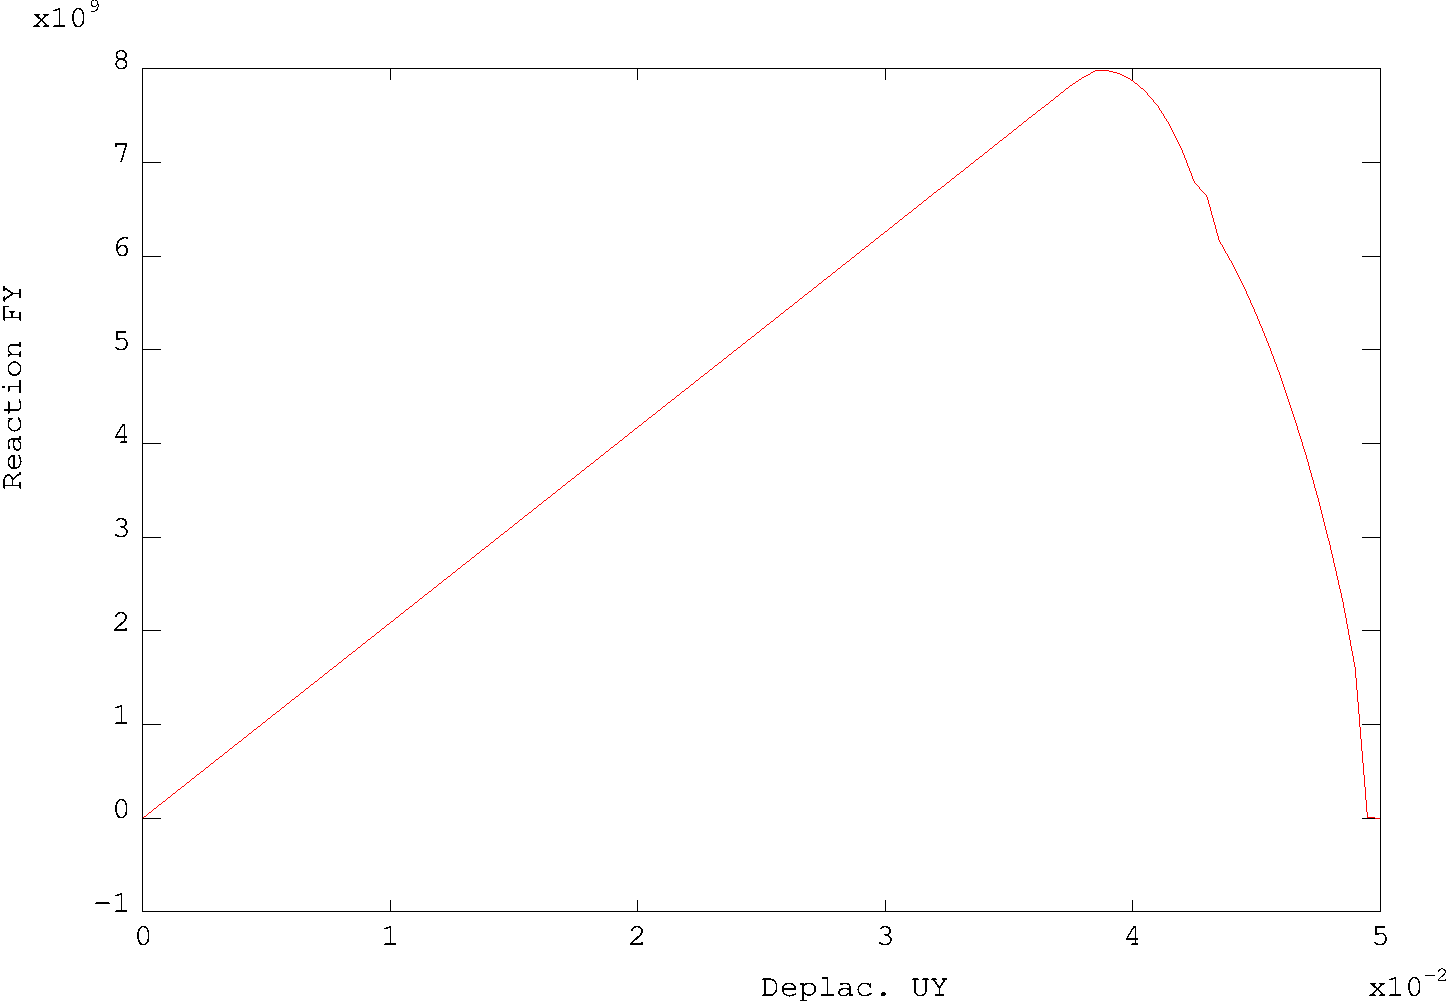
\includegraphics[height=3.5cm]{images/exo/exo_2_solu_evol}
%       \hspace{0.4cm}
%       \animategraphics[controls,loop,poster=last,height=3.5cm]{10}{images/exo/exo_2_solu_sigma.}{01}{46}
%     \end{center}
%     \item \fe{Modèle peu robuste\\ résultats très sensibles à la discrétisation espace/temps}
%              {Undependable model\\ results quite sensitive to time/space discretization}
%   \end{itemize}
% \end{frame}
